\documentclass{article}
\usepackage{stackengine}
\usepackage{graphicx}
\usepackage{cite}
\title{Lecture 1: Introduction}
\author{Shashank Vatedka}

\usepackage{basicreq}
\usepackage{./teaching_doc_macros}

\begin{document}

%FILL IN THE RIGHT INFO.
%\lecture{**LECTURE-NUMBER**}{**UNIT**}{**LECTURER**}{**SCRIBE**}
\lecture{2}{Convexity}{Shashank Vatedka}{Ritesh Kumar}
%\footnotetext{These notes are partially based on those of Nigel Mansell.}

% **** YOUR NOTES GO HERE:

% Some general latex examples and examples making use of the
% macros follow.  
%**** IN GENERAL, BE BRIEF. LONG SCRIBE NOTES, NO MATTER HOW WELL WRITTEN,
%**** ARE NEVER READ BY ANYBODY.

\section{Open set}

A set $\mathcal{A}$ is said to be an open set if for every $\underline{x} \in \mathcal{A}$, we can find $\epsilon > 0$ such that,
\begin{equation}
B_{\epsilon}(\underline{x}) \subseteq \mathcal{A}
\end{equation}
Where $B_{\epsilon}(\underline{x})$	 is an n-dimensional ball with radius $\epsilon$ and center $\underline{x}$. No matter which point we are taking , it always lies within  the set. Open sets are typically denoted as $\left( \mathcal{A}\right)$. In general we denote  open interval using $\left( \right)$. For example $\left(a, b\right)$ is open interval and $\left(4,5\right)$ $\cup$ $\left( 6,8\right)$ is an open set.
\section{Closed set}
A set $\mathcal{A}$ is said to be closed set if:
\begin{itemize}
	\item  Compliment of the set is an open set. 
	\item Every limit point of the set lies inside the set.
	\item Closed interval is  denoted as $\left[\right]$ and $\left[ a, b\right]$ $\cup$ $\left[ p, q\right]$ is closed set. But $\left(a, b\right)$ $\cup$ $\left[p, q\right]$ is neither closed set neither open set.
\end{itemize}


\section{Convex set}
$\mathcal{A}$ is said to be a convex set if, $\forall $\vspace{5pt} $\underline{x}, \underline{y} \in \mathcal{A}$ and $\forall$ \vspace{5pt} $0\leq \alpha \leq 1$ 
\begin{equation}
	\alpha \underline{x} + (1-\alpha)\underline{y} \in \mathcal{A}
\end{equation}
Geometrically, if we consider any two points inside the set, then every point that lies on the line that joins these two points must lie inside the set.
\begin{figure*}[h!]
	\centering
	\subfloat{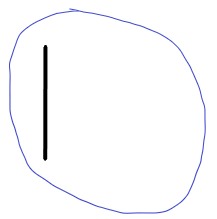
\includegraphics[height=.10\textheight]{pic2.png}} \hspace{30pt}
	\subfloat{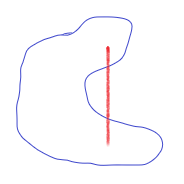
\includegraphics[height=.10\textheight]{pic1.png}}
	\caption{(a)Convex set \hspace{20pt} (b) Not a convex set} 
	\label{fig2}
\end{figure*}
\newpage
 \textbf{Example :} Achievable rate regions are convex: a time-sharing argument :
 Consider a multi-user system where we have some L-transmitter and L-receiver and they want to communicate through the channel described in figure \ref{fig3}. We want to find the achievable rate over this channel.\\ 
 \begin{figure}[htb!]
 	\centering
 	\includegraphics[height=.20\textheight]{pic3.pdf}
 	\caption{(a) Transceiver for L-transmitter and Receiver setting } 
 	\label{fig3}
 \end{figure}
 
 
 A rate tuple $\left( R_{1}, R_{2} \dots R_{L} \right)$ is achievable if $\exists$ pair of encoder and decoder. \\
 $\left( ENC_{n}(1), ENC_{n} (2), \dots ENC_{n}(L), DEC_{n}(1), DEC_{n}(2) \dots , DEC_{n}(L)\right)$  pair can be defined as :\\
 $ENC_{n}(i) :\left\{0,1\right\}^{K_{n}(i)} \longrightarrow  \mathcal{X}^{n}(l) $ and ,
 $DEC_{n}(i) : \mathcal{Y}^{n}(i) \longrightarrow \left\{ 0,1 \right\}^{K_{n}(i)}$ such that : \\
\begin{align}
	\stackunder{$\limsup$ }{$n$ $\rightarrow$ $\infty$} \frac{K_{n}(i)}{n} = R_{i}
\end{align}
\begin{align}
	\stackunder{$\limsup$ }{$n$ $\rightarrow$ $\infty$} Pr \left[ M'_{i} \neq M_{i}\right] = P_{e} = 0 \label{2.4}
\end{align}
  And we want to find what kind of rate can be achievable. Consider the tuple $\left( R_{1}, R_{2}\right)$ i.e (L = 2) which is achievable. For single T$_{X}$ - R$_{X}$ setting $\left( \text{i.e} \hspace{5pt}  L = 1 \right)$, according to the Shannon coding theorem, any rate less than the capacity of the channel is achievable. So, rate region for the single $T_{X} - R_{X} $ is a closed interval which is $\left[ 0, C \right]$.\\  \\
  \textbf{ For the 2 user case :}
  \begin{figure}[htb!]
  	\centering
  	\includegraphics[height=.25\textheight]{pic4.pdf}
  	\caption{2 user rate tuple  case ( 2 user Gaussian multiple-access channel (MAC) only)}
  \end{figure}
\newline 
\textbf{Theorm :} Every rate region are convex. i.e if   $\left( R_{1}, R_{2}\right) \& \left( R'_{1}, R'_{2}\right)$ are achievable and they lie in the rate region then $\forall$ 0$\leq$ $\alpha$ $\leq$ 1, \hspace{5pt} $\left( \alpha R_{1} + (1-\alpha)R'_{1}, \alpha R'_{2} + (1-\alpha)R_{2},   \right)$ is achievable.\\
  \begin{figure}[htb!]
	\centering
	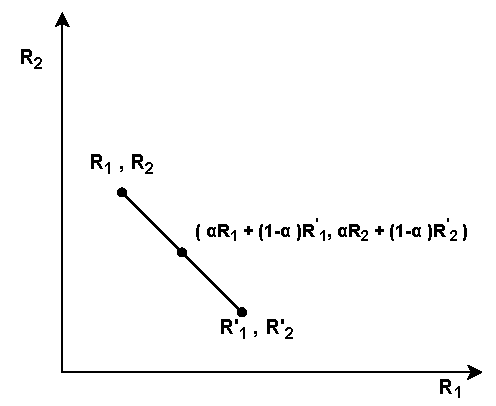
\includegraphics[height=.25\textheight]{pic5.pdf}
	\caption{2 user rate  case}
\end{figure}
\textbf{Proof :}  Consider a time sharing argument $\left(R_1, R_2 \right)$ and  $\left(R'_1, R'_2 \right)$ for ENC and DEC pair such that :\\
 $K_{n}(1) \geq n\left( R_1 - \epsilon \right)$ and $K_{n}(2) \geq n\left( R_2 - \epsilon \right)$ for $\left( ENC, DEC \right)$.
  $K'_{n}(1) \geq n\left( R'_1 - \epsilon \right)$ and $K'_{n}(2) \geq n\left( R'_2 - \epsilon \right)$ for $\left( ENC', DEC' \right)$ \\
  We have n channel uses and consider $\alpha$n  channel uses by first  $\left( ENC-DEC \right)$ pair and $\left(1 -\alpha \right)n$ for  $\left( ENC'-DEC' \right)$ pair. Hence
  \begin{equation}
  	  \alpha K_{n}(1) \geq \alpha n\left( R_1 - \epsilon \right) \label{2.5}
  	\end{equation}
    \begin{equation}
\alpha K_{n}(2) \geq   \alpha n\left( R_2 - \epsilon \right) \label{2.6}
  \end{equation}
 and,
  
  \begin{equation}
	\left(1 - \alpha  \right)  K'_{n}(1) \geq \left(1 - \alpha  \right) n\left( R'_1 - \epsilon \right) \label{2.7}
\end{equation}
\begin{equation}
	\left(1 - \alpha  \right) K'_{n}(2) \geq   \left(1 - \alpha  \right)n\left( R'_2 - \epsilon \right) \label{2.8}
\end{equation}
   Combining \eqref{2.5}, \eqref{2.7} and \eqref{2.6}, \eqref{2.8}, we have 
 
\begin{equation}
	\alpha K_{n}(1)	+ \left(1 - \alpha  \right) K'_{n}(1) \geq   \alpha n\left( R_1 - \epsilon \right) +  \left(1 - \alpha  \right)n\left( R'_1 - \epsilon \right) \label{2.9
	}
\end{equation}   
  
\begin{equation}
 \alpha K_{n}(2)	+ \left(1 - \alpha  \right) K'_{n}(2) \geq   \alpha n\left( R_2 - \epsilon \right) +  \left(1 - \alpha  \right)n\left( R'_2 - \epsilon \right) \label{2.10}
\end{equation}  
  
 And it holds $\forall$ $\epsilon > 0 $.\\ 
%  Using Fano's inequality we can  prove the equation \eqref{2.4}. We can have,\\
%  \begin{equation}
%  K_{n} \leq H_{2}(P_{e}) + P_{e}log_{2}(2^{M^{K_{n}}}) + I(M^{K_{n}}:{M'}^{K_{n}})
%  \end{equation}
%Where, P$_{e} = \stackunder{$\limsup$ }{$n$ $\rightarrow$ $\infty$} Pr \left[ M'_{i} \neq M_{i}\right]$
%  \begin{equation}
%   K_{n} \leq H_{2}(P_{e}) + P_{e}log_{2}(2^{{K_{n}}}) + I(X^{n} : Y^{n}) \text{\hspace{5pt}(using data processing inequality)}
%  \end{equation}
%\begin{figure}
% \centering
%\includegraphics[height=.05\textheight]{pic6.pdf}
%\caption{ Single user transmission system }
%\end{figure}
%  \begin{align}
%  	K_{n} \leq H_{2}(P_{e}) + P_{e}K_{n} + I(X^{n} : Y^{n})
%  \end{align}
%  \begin{eqnarray*}
%  	K_{n}  \leq H_{2}(P_{e}) + P_{e}K_{n} + nC  \Rightarrow \frac{H_{2}(P_{e})}{n} \geq \frac{K_{n}(1 - P_{e})}{n} - C \\
% 	\stackunder{$\lim$ }{$n$ $\rightarrow$ $\infty$} \left(  \frac{K_{n}(1 - P_{e})}{n} - C \right) \leq  \stackunder{$\lim$ }{$n$ $\rightarrow$ $\infty$} \frac{H_{2}(P_{e})}{n}  
% \end{eqnarray*} 
%Let $\frac{K_{n}}{n} = R $, \\
% 
%\begin{align}
%\stackunder{$\lim$}{$n$ $\rightarrow$ $\infty$} P_{e} \geq \frac{R - C}{R} 
%\end{align}
% 
% \begin{align}
% 	\stackunder{$\limsup$}{$n$ $\rightarrow$ $\infty$} P_{e} \geq \frac{R - C}{R} \label{2.15}
% \end{align} 
%  
%  If we operate at the rate more than capacity of the channel say R = C + $\epsilon$
%  \begin{align}
%  	\stackunder{$\limsup$}{$n$ $\rightarrow$ $\infty$} \hspace{5pt} P_{e} \geq \frac{\epsilon}{R} 
%  \end{align}
%That is probability or error  is always non-zero.But if we operate the channel  below the capacity and for large n, in \eqref{2.15} we can observe P$_{e}$  approaches to 0.  
%  
%  
Now consider, we have pair of encoder and decoder $\left( ENC, DEC\right)$ and $\left( ENC', DEC'\right)$. First pair of encoder and decoder transmit $\alpha$k$_{1}$  bits in $\alpha$n channel use. And receiver received $\alpha$n symbols. Similarly second pair of  encoder and decoder transmit $ \left (1 - \alpha \right)$k$_{2}$  bits in $ \left( 1 -\alpha \right)$n channel use. And receiver received $\alpha$n symbols. \\ Overall rate of this setting is give as :
\begin{equation} 
	\text{Rate} = \frac{ \alpha \text{k}_1 + (1 - \alpha)\text{k}_2}{\text{n}}
\end{equation}
Suppose the probability of error for channel first pair of ENC - DEC is $P_{e1}$ and for the second pair is $P_{e2}$, then
For this the overall probability of error  is :
\begin{equation}
	P_e = P_{e1} + P_{e2} -( P_{e1} \cap P_{e2})  \label{2.12}
\end{equation}
Since both are independent.
\begin{align}
	P_e = P_{e1} + P_{e2} - P_{e1}.P_{e2}  \label{2.13} \\
	\Rightarrow P_{e} \leq P_{e1} + P_{e2} \label{2.14}
\end{align}
Where $P_{e1} = P_{e}^{\alpha \text{n}}$, $P_{e2} = P_{e}^{\left (1 - \alpha \right ) \text{n}}$ 
As we know, if n is sufficiently large, $P_{e1}$ and $P_{e2}$ asymptotically approaches to zero. Hence from \ref{2.12}, we can observe the overall probability of error will be zero.



 
  
  
  
  
\end{document}

